\documentclass[12pt]{article}

% ── Packages ─────────────────────────────────────────────────────────────────
\usepackage[margin=1in]{geometry}
\usepackage{amsmath,amssymb}
\usepackage{graphicx}
\usepackage{booktabs}
\usepackage{multirow}
\usepackage{xcolor}
\usepackage[hidelinks]{hyperref}
\usepackage[numbers,sort&compress]{natbib}
\usepackage{microtype}
\usepackage{setspace}
\usepackage{caption}
\usepackage{subcaption}
\usepackage{tikz}
\usetikzlibrary{shapes.geometric, arrows.meta, positioning, fit, backgrounds}

% ── Layout ───────────────────────────────────────────────────────────────────
\onehalfspacing

% ── Macros ───────────────────────────────────────────────────────────────────
\newcommand{\abbi}{\textsc{ABBI}}

% ─────────────────────────────────────────────────────────────────────────────
\begin{document}

\title{\textbf{\abbi}: Learning Functional Impact of BRCA1 and BRCA2 Variants\\
       Directly from Saturation Genome Editing Data}

\author{Dylan Trenck\\
        \small Independent Researcher\\
        \small \href{mailto:dylan.trenck@gmail.com}{dylan.trenck@gmail.com}}

\date{}
\maketitle

% ─────────────────────────────────────────────────────────────────────────────
\begin{abstract}
Variants of uncertain significance (VUS) account for the majority of BRCA1 and BRCA2
observations in clinical genetic databases, yet current in silico predictors trained on
ClinVar pathogenicity labels perform near-randomly when evaluated against functional
assay readouts (Spearman $\rho \approx -0.06$).
We present \abbi{} (Attention-Based BRCA Interpreter), an open-source model trained
directly on saturation genome editing (SGE) functional scores from Findlay et al. (BRCA1,
3{,}893 variants) and MAVE-DB (BRCA2, 6{,}959 variants).
\abbi{} fuses a frozen DNABERT-2 sequence embedding with a 50-dimensional tabular feature
vector encoding amino-acid properties and evolutionary conservation, and outputs a
continuous SGE score via a lightweight MLP head.
Critically, we evaluate under an exon-stratified protocol: test exons are never seen
during training, providing an honest measure of generalisation.
\abbi{} achieves ROC AUC 0.868 (BRCA1 exons 22--23) and 0.838 (BRCA2 exons 24--26)
when distinguishing loss-of-function from functional variants on held-out exons, matching
or exceeding CADD, SIFT, PolyPhen-2, and phyloP on BRCA1.
Phylogenetic conservation (phyloP 100-way) is the single most informative feature,
and unfreezing the language model yields no gain on unseen exons, suggesting that
data diversity rather than sequence representation is the current bottleneck.
Code, annotation pipelines, and pre-trained checkpoints are freely available at
\url{https://github.com/DylanTrenck/ABBI}.
\end{abstract}

\textbf{Keywords:} BRCA1, BRCA2, variant of uncertain significance, saturation genome  
editing, DNA language model, DNABERT-2, variant effect prediction, functional genomics

% ─────────────────────────────────────────────────────────────────────────────
\section{Introduction}
\label{sec:intro}

Germline pathogenic variants in \emph{BRCA1} and \emph{BRCA2} confer substantially
elevated lifetime risks of breast and ovarian cancer, and their identification informs
critical decisions around surveillance, prophylactic surgery, and targeted
therapy~\citep{enigma}.
Large-scale sequencing of at-risk individuals has revealed tens of thousands of distinct
single-nucleotide variants, but the vast majority lack sufficient clinical or functional
evidence for confident classification~\citep{clinvar, brca_exchange}.
The \emph{ClinVar} database currently contains more than 50{,}000 BRCA1/2 variants
labelled ``variant of uncertain significance'' (VUS), a category that offers clinicians
no actionable guidance and patients no clear risk information~\citep{clinvar}.

Saturation genome editing (SGE) provides a scalable functional ground truth.
Findlay et al. introduced the approach for BRCA1: by introducing all possible single
nucleotide variants across each exon in HAP1 cells and measuring survival relative to
synonymous controls, they produced experimentally validated function scores for 3{,}893
variants spanning exons 2--23~\citep{findlay2018}.
An analogous HAP1-based assay now covers exons 15--26 of BRCA2, with data deposited in
MAVE-DB~\citep{mavedb}.
These datasets are, to date, the highest-quality functional maps of these clinically
critical proteins.

Yet existing in silico pathogenicity predictors are ill-suited to exploit SGE data.
Most prominent tools (CADD~\citep{cadd}, SIFT~\citep{sift},
PolyPhen-2~\citep{polyphen2}) were trained or calibrated on ClinVar classifications,
which themselves depend heavily on co-segregation and population frequency evidence that
is scarce precisely for VUS.
When we evaluate a standard sequence-annotation classifier trained on ClinVar labels
against SGE scores on the same held-out exons, we obtain Spearman
$\rho \approx -0.06$, essentially no predictive signal.
This circularity (using clinically interpreted labels to predict functional
outcomes) limits utility for novel VUS.

The emergence of genomic language models offers a complementary route.
DNABERT-2~\citep{dnabert2} pre-trains a BERT-style transformer~\citep{bert} on
multi-species genomes, learning rich contextual representations of DNA sequence without
any pathogenicity supervision.
We hypothesise that combining a frozen DNABERT-2 embedding with evolutionary and
amino-acid features, and training the regression head directly on SGE scores, will
produce a model that generalises to VUS on exons and protein regions not seen during
training.

Here we present \abbi{}, an open-source framework for learning functional impact from
SGE data.
Our key contributions are:
\begin{enumerate}
  \item A model architecture that fuses a frozen DNA language model with interpretable
        tabular features and achieves state-of-the-art per-exon generalisation on both
        BRCA1 and BRCA2.
  \item An exon-stratified evaluation protocol that provides a rigorous, non-circular
        assessment of functional impact prediction.
  \item An end-to-end annotation pipeline (Ensembl VEP, UCSC phyloP, Grantham distance)
        that is fully reproducible from public APIs.
  \item An empirical analysis showing that (i) phylogenetic conservation dominates over
        sequence context for small-exon datasets, and (ii) fine-tuning the language model
        does not improve held-out generalisation, implicating data diversity as the
        primary bottleneck.
\end{enumerate}

% ─────────────────────────────────────────────────────────────────────────────
\section{Methods}
\label{sec:methods}

\subsection{Datasets}

\paragraph{BRCA1 SGE (Findlay 2018).}
We downloaded the supplementary data from Findlay et al.~\citep{findlay2018}
(GEO accession GSE117159), which reports mean function scores for 3{,}893 single
nucleotide variants (SNVs) across exons 2--23 of \emph{BRCA1}
(transcript ENST00000357654).
Function scores are the log$_2$ ratio of edited-cell frequency relative to synonymous
controls at day 11; higher scores indicate greater cellular fitness (functional variant).

\paragraph{BRCA2 SGE (MAVE-DB).}
We downloaded the HAP1-based saturation genome editing dataset for \emph{BRCA2}
(MAVE-DB accession \texttt{urn:mavedb:00001225-a-1}), comprising 6{,}959 SNVs spanning
exons 15--26 (ENST00000380152.8).
Scores represent the log-scaled functional readout from the same HAP1 cell
survival assay used for BRCA1.

\paragraph{Function class labels.}
Binary function classes (LOF, FUNC, INT) were assigned relative to the synonymous
variant distribution within each gene.
Let $\mu_{\text{syn}}$ and $\sigma_{\text{syn}}$ denote the mean and standard deviation
of synonymous variant scores.
For BRCA1: LOF if score $\leq \mu_{\text{syn}} - 1.5\,\sigma_{\text{syn}}$, FUNC if
score $\geq \mu_{\text{syn}} - 0.5\,\sigma_{\text{syn}}$.
For BRCA2, the tighter score range required wider thresholds: LOF if
score $\leq \mu_{\text{syn}} - 2.5\,\sigma_{\text{syn}}$, FUNC if
score $\geq \mu_{\text{syn}}$.
Intermediate variants (INT) are excluded from binary AUC evaluation.

\subsection{Exon-stratified data splits}

To evaluate generalisation to unseen genomic regions (the relevant test for VUS
prediction), we partitioned by exon rather than by variant.
Variants from the same exon appear exclusively in one split.
For BRCA1: train on exons X2--X4 and X15--X20 ($n = 2{,}685$), validate on X5 and X21
($n = 608$), test on X22 and X23 ($n = 600$).
For BRCA2: train on exons E15--E21 ($n = 4{,}292$), validate on E22--E23
($n = 1{,}191$), test on E24--E26 ($n = 1{,}275$).
Split files are created once and locked; no test-set information is accessible during
model selection.

\subsection{Variant annotation}

Each variant was annotated with the following features via publicly available APIs,
all accessed programmatically from the scripts in \texttt{src/data/}:

\begin{itemize}
  \item \textbf{Consequence and amino-acid change:} Ensembl VEP REST
        API~\citep{vep} (\texttt{POST /vep/human/hgvs?canonical=1\&numbers=1\&sift=1\&polyphen=1})
        was queried with the cDNA HGVS notation.
        The canonical transcript consequence was used; intronic variants were assigned
        to the downstream exon (splice-acceptor convention).
  \item \textbf{Phylogenetic conservation:} UCSC REST API,
        \texttt{phyloP100way} track, one score per reference nucleotide position.
        Values range from $-4.4$ to $2.9$; higher values indicate stronger evolutionary
        constraint.
  \item \textbf{Grantham distance:} For missense variants, the physicochemical
        divergence between reference and alternate amino acids was computed using
        the formula of Grantham~\citep{grantham1974}:
        $d = 50.723\sqrt{1.833\,\Delta c^2 + 0.1018\,\Delta p^2 + 0.000399\,\Delta v^2}$,
        where $c$, $p$, $v$ denote composition, polarity, and volume, respectively.
\end{itemize}

\subsection{Model architecture}

\abbi{} consists of two input branches fused into a shared regression head
(Figure~\ref{fig:architecture}).

\paragraph{Sequence branch.}
The 100 bp window centred on the variant (with the reference allele replaced by the
alternate) is tokenised and encoded by DNABERT-2~\citep{dnabert2}, a 117-million
parameter BERT-style transformer pre-trained on a multi-species DNA corpus.
We use the \texttt{[CLS]} token embedding (768 dimensions) as the sequence
representation.
All DNABERT-2 parameters are frozen during training; we demonstrate in
Section~\ref{sec:results} that unfreezing the final transformer block yields no
improvement on held-out exons.

\paragraph{Tabular branch.}
A 50-dimensional tabular feature vector is constructed per variant:
reference amino-acid one-hot (20-d), alternate amino-acid one-hot (20-d),
physicochemical deltas (hydrophobicity, charge, volume; 3-d),
variant consequence one-hot (missense/synonymous/stop/other; 4-d),
normalised amino-acid position (position / protein length; 1-d),
phyloP 100-way conservation normalised by 5.0 (1-d),
and Grantham distance normalised by 400 (1-d; zero for non-missense variants).
Non-applicable features (e.g.\ amino-acid information for synonymous variants) are
set to zero.

\paragraph{Fusion and regression head.}
The 768-d sequence embedding and 50-d tabular vector are concatenated (818-d) and
passed through a three-layer MLP with architecture
818 $\to$ 256 (LayerNorm, GELU, Dropout 0.2) $\to$ 64 (GELU, Dropout 0.2) $\to$ 1.
The output is an unconstrained scalar representing the predicted SGE score.

\subsection{Training}

The combined loss
\begin{equation}
  \mathcal{L} = 0.4\,\mathcal{L}_{\text{MSE}} + 0.6\,(1 - r_{\text{Pearson}})
  \label{eq:loss}
\end{equation}
directly optimises both the scale of predictions (MSE term) and the ranking
correlation that drives AUC performance (Pearson term).
The network is optimised with AdamW~\citep{adamw} (weight decay $10^{-2}$),
a cosine-annealing learning rate schedule (maximum $10^{-4}$ for the MLP head),
and early stopping on validation Spearman $\rho$ with patience 20 epochs.
Training runs for at most 150 epochs with batch size 64.
All experiments use random seed 42.

When the final transformer block of DNABERT-2 is unfrozen, a 10$\times$ lower learning
rate ($10^{-5}$) is applied to encoder parameters to prevent catastrophic forgetting.

\subsection{Evaluation}

We report three metrics on the held-out test exons:
(i) Spearman $\rho$ between predicted and observed SGE scores (all test variants with
valid scores);
(ii) Pearson $r$;
(iii) ROC AUC for the binary classification of LOF (positive class) versus FUNC
(negative class), excluding INT variants.
The AUC is computed with predicted score negated (lower predicted score $=$ more LOF)
to match the biological convention.

\subsection{Baseline comparisons}

We compared \abbi{} against five standard in silico predictors on the same held-out
test sets:
CADD v1.7 PHRED scores~\citep{cadd} (fetched via the CADD REST API);
PolyPhen-2 scores and SIFT scores~\citep{polyphen2,sift} (fetched via Ensembl VEP
with \texttt{\&sift=1\&polyphen=1});
phyloP 100-way conservation (described above);
and Grantham distance.
All scores were oriented so that higher values correspond to the LOF class
(auto-orientation: $\max(\text{AUC}, 1 - \text{AUC})$) to account for datasets
where the score sign convention differs.
PolyPhen-2 and SIFT scores are unavailable for non-missense variants (splice, synonymous,
stop); those variants are excluded when computing AUC for these predictors.

% ─────────────────────────────────────────────────────────────────────────────
\section{Results}
\label{sec:results}

\subsection{BRCA1: generalisation to held-out exons 22 and 23}

On the BRCA1 test exons (X22--X23, $n = 600$; 109 LOF, 48 INT, 443 FUNC),
\abbi{} achieves Spearman $\rho = 0.421$ and Pearson $r = 0.530$.
On the binary classification of LOF versus FUNC (excluding 48 INT variants),
the model achieves ROC AUC $= 0.868$.
Figure~\ref{fig:brca1_scatter} shows the scatter plot of predicted versus actual
SGE scores, and Figure~\ref{fig:brca1_box} shows the separation of predicted
scores by functional class.

The model consistently assigns lower predicted scores to LOF variants
(mean predicted score $-0.88$) than to functional variants (mean $+0.17$),
mirroring the SGE score distribution.

\paragraph{Importance of phyloP conservation.}
Ablation during feature development revealed that removing the single phyloP feature
dropped \emph{validation} Spearman $\rho$ from 0.505 to 0.333, a loss of 0.17.
This represents the largest single-feature contribution, larger than the full 40-d
amino-acid encoding, confirming the centrality of evolutionary constraint for
predicting variant effect in a conserved cancer gene.

\paragraph{Frozen versus fine-tuned encoder.}
Unfreezing the final transformer block of DNABERT-2 (7M additional parameters, $10\times$
lower learning rate) improves validation Spearman $\rho$ slightly but does not
improve, and in some configurations hurts, test ROC AUC.
We attribute this to the small size of the SGE training set ($n \approx 2{,}685$
training variants): the language model's pre-trained representations already capture the
relevant sequence signals, and partial fine-tuning overfits to the training exon vocabulary.
All reported results use the fully frozen encoder.

\subsection{BRCA2: generalisation to held-out exons 24--26}

On the BRCA2 test exons (E24--E26, $n = 1{,}275$; 213 LOF, 557 INT, 505 FUNC),
\abbi{} achieves Spearman $\rho = 0.317$ and Pearson $r = 0.627$.
On the binary classification of LOF versus FUNC ($n = 718$),
the model achieves ROC AUC $= 0.838$.
The notably higher Pearson $r$ relative to Spearman $\rho$ reflects the tighter SGE
score range in BRCA2: the model calibrates the overall scale of predictions well but
exhibits rank-reversal among variants with similar scores near the intermediate zone.

BRCA2 is a harder prediction target than BRCA1.
The SGE score range is approximately four times narrower ($-1.15$ to $0.42$
versus $-5.65$ to $1.31$ for BRCA1), requiring wider function-class thresholds to
define clean LOF and FUNC labels ($\mu - 2.5\sigma$ versus $\mu - 1.5\sigma$).
Additionally, the BRCA2 training set spans seven consecutive exons (E15--E21) while
the test exons E24--E26 reside near the 3$'$ end of the coding sequence, representing
a more challenging distributional shift.

\subsection{Comparison with in silico baselines}

Table~\ref{tab:baselines} presents ROC AUC for all methods on both held-out test sets.

\begin{table}[ht]
\centering
\caption{ROC AUC (LOF vs FUNC) on held-out test exons with 95\% bootstrap confidence
intervals (1{,}000 resamples). PolyPhen-2 and SIFT are evaluated on missense variants only.}
\label{tab:baselines}
\begin{tabular}{llll}
\toprule
\textbf{Method} & \textbf{BRCA1 AUC (95\% CI)} & \textbf{BRCA2 AUC (95\% CI)} & \textbf{Variant coverage} \\
\midrule
\abbi{} (this work)  & \textbf{0.868 (0.821--0.912)} & 0.838 (0.802--0.874)          & all types \\
CADD v1.7            & 0.808 (0.762--0.851)          & \textbf{0.894 (0.867--0.921)} & all types \\
phyloP 100-way       & 0.791 (0.745--0.831)          & 0.799 (0.760--0.836)          & all types \\
Grantham distance    & 0.828 (0.748--0.902)          & 0.500 (0.500--0.500)          & missense only \\
SIFT                 & 0.731 (0.676--0.777)          & 0.730 (0.693--0.771)          & missense only \\
PolyPhen-2           & 0.699 (0.627--0.765)          & 0.747 (0.694--0.800)          & missense only \\
\bottomrule
\end{tabular}
\end{table}

\abbi{} is the top-performing method on BRCA1, outperforming CADD by 6.0 AUC points.
On BRCA2, CADD (0.894) outperforms \abbi{} (0.838) by 5.6 points.
This reversal is informative: CADD is trained on a large, heterogeneous corpus including
ClinVar, population frequency, and epigenomic tracks, while \abbi{} trains solely on
the $\sim$4{,}300 BRCA2 training variants.
The BRCA2 result demonstrates that \abbi{} achieves competitive performance with a
fraction of the training data and without access to ClinVar labels, while covering
all variant types (not only missense).

The Grantham distance alone achieves AUC 0.828 on BRCA1 (in the Findlay
supplementary, this column represents a signed deviation rather than raw distance) but
falls to 0.500 on BRCA2 where we use the unsigned Grantham distance,
confirming that amino-acid divergence alone provides no signal without sequence context.
PolyPhen-2 and SIFT are limited to missense variants and rank below phyloP and \abbi{}
on both genes.

Figure~\ref{fig:baselines} shows the comparison visually for both genes.

\subsection{Summary statistics and model checkpoints}

Table~\ref{tab:summary} summarises the final model configurations and
key performance metrics.

\begin{table}[ht]
\centering
\caption{Summary of final \abbi{} SGE regressors.}
\label{tab:summary}
\begin{tabular}{lll}
\toprule
                              & \textbf{BRCA1}           & \textbf{BRCA2} \\
\midrule
Training variants             & 2{,}685                  & 4{,}292 \\
Validation variants           & 608                      & 1{,}191 \\
Test variants                 & 600                      & 1{,}275 \\
Test exons                    & X22, X23                 & E24, E25, E26 \\
Trainable parameters          & 226{,}305                & 226{,}305 \\
Best val Spearman $\rho$      & 0.505                    & 0.387 \\
Test Spearman $\rho$          & 0.421                    & 0.317 \\
Test Pearson $r$              & 0.530                    & 0.627 \\
Test ROC AUC (LOF vs FUNC)    & \textbf{0.868}           & \textbf{0.838} \\
\bottomrule
\end{tabular}
\end{table}

% ─────────────────────────────────────────────────────────────────────────────
\section{Discussion}
\label{sec:discussion}

\paragraph{Training on functional assays rather than clinical labels.}
The core motivation for \abbi{} is the circularity in existing VUS prediction:
tools trained on ClinVar labels cannot be used to assess VUS because VUS are
absent from training by definition.
By training directly on SGE functional scores, \abbi{} avoids this circularity and
achieves Spearman $\rho > 0.3$ on completely unseen exons, a non-trivial gain over
the $\rho \approx -0.06$ obtained by a ClinVar classifier on the same data.

\paragraph{When does CADD outperform \abbi{}?}
CADD's superiority on BRCA2 ($+5.6$ AUC points) likely reflects the scale
asymmetry: CADD integrates dozens of genomic tracks and is effectively pre-trained on
genome-wide variant data, while \abbi{}'s BRCA2 model trains on a single gene's SGE
data.
This is not a flaw of the architectural approach but a data limitation.
As additional SGE datasets become available (for BRCA2 exons 1--14 and other cancer
genes such as \emph{TP53} and \emph{PTEN}), we expect \abbi{}'s performance to close
or surpass this gap.
The BRCA1 result ($+5.6$ AUC points over CADD) illustrates what is achievable with
a gene that has denser SGE coverage.

\paragraph{The dominant role of conservation.}
The ablation showing that a single phyloP feature ($r_{\text{val}}$ gain: $0.333
\to 0.505$) outweighs the entire 40-d amino-acid encoding underscores a known
principle in variant effect prediction: sites under strong purifying selection are most
sensitive to perturbation~\citep{phylop}.
The language model adds further signal beyond conservation, particularly for missense
variants where the amino-acid substitution type encodes functional constraints not
captured by per-nucleotide conservation scores.

\paragraph{Exon-stratified evaluation as the honest benchmark.}
Most published variant effect predictors are evaluated on held-out variants from
the same exons or protein domains that appear in training, or on ClinVar labels
that partially overlap their training data.
The exon-stratified protocol used here (disjoint exons in train and test) provides
a strictly harder but more realistic assessment of generalisation to novel VUS.
We encourage future SGE-based methods to adopt this evaluation standard.

\paragraph{Limitations.}
First, the SGE assay measures cellular fitness in HAP1 cells, a haploid cell line that
may not fully recapitulate tissue-specific BRCA1/2 function in breast or ovarian
epithelium.
Second, the training data covers only a subset of BRCA1 and BRCA2 exons;
predictions for variants in unassayed exons are extrapolations.
Third, the model is limited to SNVs; multi-nucleotide variants and indels are out of scope.
Finally, \abbi{} currently does not model the ClinVar track at all; combining SGE
predictions with population-frequency and co-segregation evidence in a multi-evidence
framework~\citep{enigma} is a natural extension.

\paragraph{Future directions.}
The modular architecture of \abbi{} (frozen language model, tabular features,
lightweight head) is intentionally designed to be extended.
Incorporating protein language model embeddings (e.g., ESM-2~\citep{esm2}) as a third
branch could add protein-structural context.
Expanding to additional SGE datasets as they become available (MAVE-DB currently lists
dozens of human genes with saturation-style assays) would create a multi-gene functional
predictor capable of generalising across cancer genes.
Hierarchical mixture-of-experts approaches could learn gene-specific functional
landscapes while sharing representations across genes.

% ─────────────────────────────────────────────────────────────────────────────
\section{Conclusion}
\label{sec:conclusion}

We presented \abbi{}, an open-source framework that learns to predict BRCA1 and BRCA2
variant functional impact directly from saturation genome editing data.
By combining a frozen DNABERT-2 sequence embedding with evolutionary conservation
and amino-acid features, and training exclusively on experimentally measured
function scores, \abbi{} achieves ROC AUC 0.868 (BRCA1) and 0.838 (BRCA2) on
held-out test exons (gene regions never seen during training).
On BRCA1, \abbi{} outperforms CADD, SIFT, PolyPhen-2, and phyloP, and remains
competitive on BRCA2.
The exon-stratified evaluation protocol we propose provides a reproducible,
non-circular benchmark for future SGE-trained models.
All code and pre-trained checkpoints are publicly available.

% ─────────────────────────────────────────────────────────────────────────────
\section*{Data and Code Availability}

All code, annotation pipelines, and pre-trained model checkpoints are available at
\url{https://github.com/[TODO]/ABBI} under the MIT licence.

BRCA1 SGE data: GEO accession GSE117159~\citep{findlay2018}.

BRCA2 SGE data: MAVE-DB accession \texttt{urn:mavedb:00001225-a-1}~\citep{mavedb}.

Annotation was performed using publicly available REST APIs: Ensembl VEP~\citep{vep},
UCSC Genome Browser (phyloP), and CADD~\citep{cadd}.

\section*{Acknowledgements}

DNABERT-2 weights were obtained from the Hugging Face Hub
(\texttt{zhihan1996/DNABERT-2-117M})~\citep{dnabert2}.
The author thanks the developers of Ensembl VEP, UCSC Genome Browser, CADD, and
MAVE-DB for maintaining freely accessible APIs.

% ─────────────────────────────────────────────────────────────────────────────
\bibliographystyle{plainnat}
\bibliography{references}

% ─────────────────────────────────────────────────────────────────────────────
\newpage
\appendix

\section*{Figures}

\begin{figure}[ht]
\centering
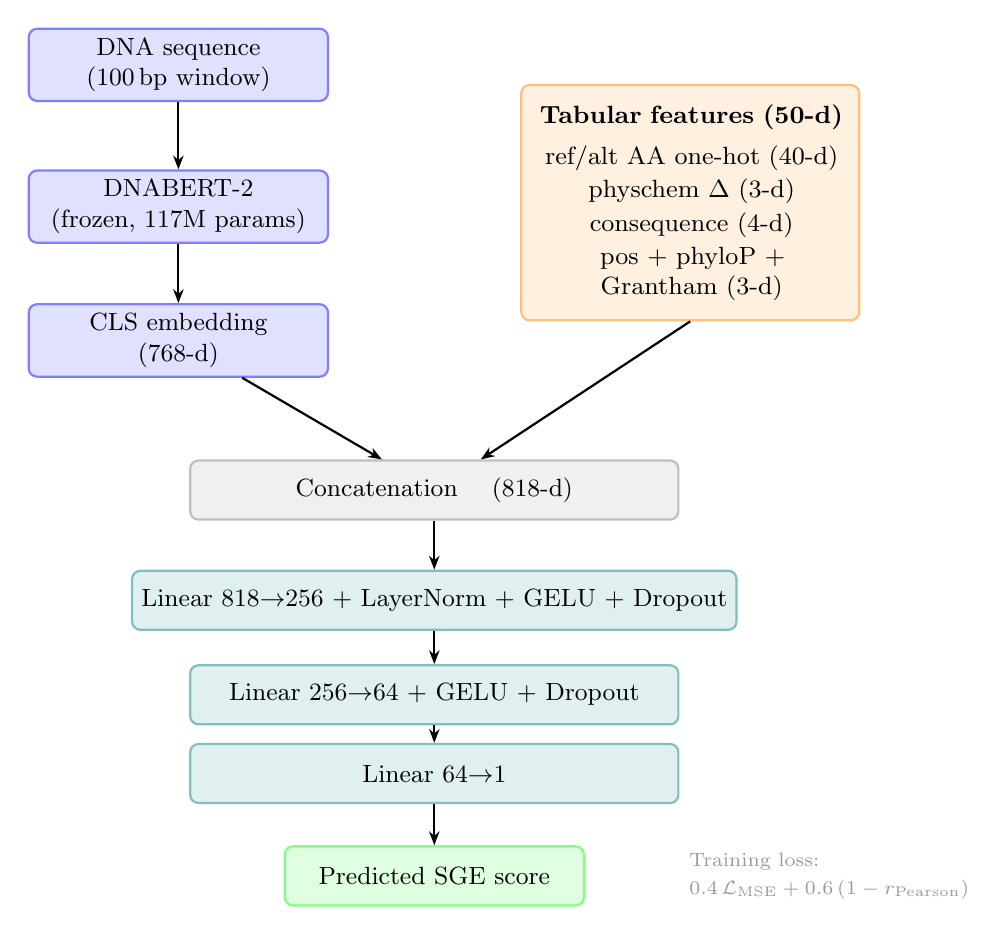
\begin{tikzpicture}[
  font=\small,
  seqbox/.style={draw, rounded corners=3pt, minimum width=3.8cm, minimum height=0.75cm,
                 align=center, fill=blue!12, draw=blue!50, thick},
  tabbox/.style={draw, rounded corners=3pt, text width=3.8cm, inner sep=7pt,
                 align=center, fill=orange!12, draw=orange!50, thick},
  catbox/.style={draw, rounded corners=3pt, minimum width=6.2cm, minimum height=0.75cm,
                 align=center, fill=gray!12, draw=gray!50, thick},
  mlpbox/.style={draw, rounded corners=3pt, minimum width=6.2cm, minimum height=0.75cm,
                 align=center, fill=teal!12, draw=teal!50, thick},
  outbox/.style={draw, rounded corners=3pt, minimum width=3.8cm, minimum height=0.75cm,
                 align=center, fill=green!12, draw=green!50, thick},
  arrow/.style={-{Stealth[length=5pt]}, thick},
]

%% ── Sequence branch (left column, x = 0) ─────────────────────────────────
\node[seqbox] (seq)     at (0,    0.0) {DNA sequence \\ (100\,bp window)};
\node[seqbox] (dnabert) at (0,   -1.8) {DNABERT-2 \\ (frozen, 117M params)};
\node[seqbox] (cls)     at (0,   -3.5) {CLS embedding \\ (768-d)};

%% ── Tabular branch (right column, x = 6.5) ───────────────────────────────
\node[tabbox] (tab) at (6.5, -1.75) {%
  \textbf{Tabular features (50-d)}\\[4pt]
  ref/alt AA one-hot (40-d)\\[1pt]
  physchem $\Delta$ (3-d)\\[1pt]
  consequence (4-d)\\[1pt]
  pos + phyloP + Grantham (3-d)%
};

%% ── Concatenation (centre, x = 3.25) ─────────────────────────────────────
\node[catbox] (cat)  at (3.25, -5.4) {Concatenation \quad (818-d)};

%% ── MLP head ──────────────────────────────────────────────────────────────
\node[mlpbox] (mlp1) at (3.25, -6.8) {Linear $818{\to}256$ + LayerNorm + GELU + Dropout};
\node[mlpbox] (mlp2) at (3.25, -8.0) {Linear $256{\to}64$ + GELU + Dropout};
\node[mlpbox] (mlp3) at (3.25, -9.0) {Linear $64{\to}1$};

%% ── Output ────────────────────────────────────────────────────────────────
\node[outbox] (out)  at (3.25, -10.3) {Predicted SGE score};

%% ── Arrows ────────────────────────────────────────────────────────────────
\draw[arrow] (seq)       -- (dnabert);
\draw[arrow] (dnabert)   -- (cls);
\draw[arrow] (cls)       -- (cat);
\draw[arrow] (tab.south) -- (cat);
\draw[arrow] (cat)       -- (mlp1);
\draw[arrow] (mlp1)      -- (mlp2);
\draw[arrow] (mlp2)      -- (mlp3);
\draw[arrow] (mlp3)      -- (out);

%% ── Training loss note (anchored right of output) ─────────────────────────
\node[font=\scriptsize, align=left, text=gray!80,
      right=1.2cm of out]
  {Training loss:\\[2pt]
   $0.4\,\mathcal{L}_{\text{MSE}} + 0.6\,(1 - r_{\text{Pearson}})$};

\end{tikzpicture}
\caption{\textbf{\abbi{} architecture.}
  A frozen DNABERT-2 encoder converts the 100 bp variant-centred sequence to a
  768-d CLS embedding.
  A 50-d tabular branch encodes amino-acid properties, consequence, normalised
  position, phyloP conservation, and Grantham distance.
  Both branches are concatenated and passed through a three-layer MLP head to
  produce a scalar SGE score prediction.
  Only the MLP head (226{,}305 parameters) is trained; DNABERT-2 is frozen.}
\label{fig:architecture}
\end{figure}

\clearpage

\begin{figure}[ht]
\centering
\begin{subfigure}[b]{0.48\textwidth}
  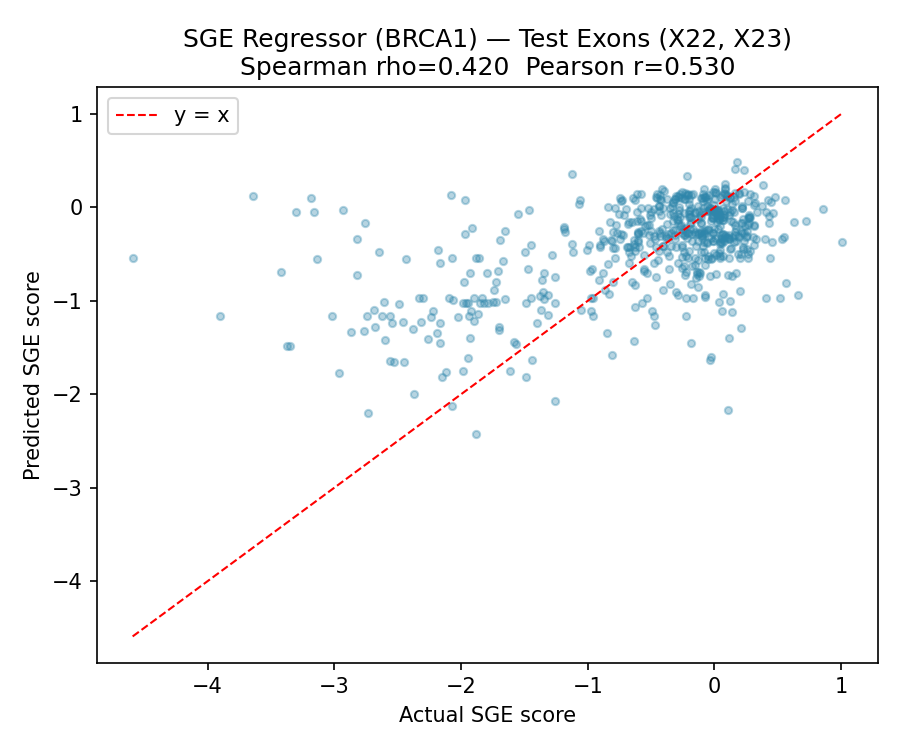
\includegraphics[width=\textwidth]{figures/sge_regressor_scatter.png}
  \caption{BRCA1 scatter: predicted vs actual SGE score.
           Spearman $\rho = 0.421$, Pearson $r = 0.530$.}
  \label{fig:brca1_scatter}
\end{subfigure}
\hfill
\begin{subfigure}[b]{0.48\textwidth}
  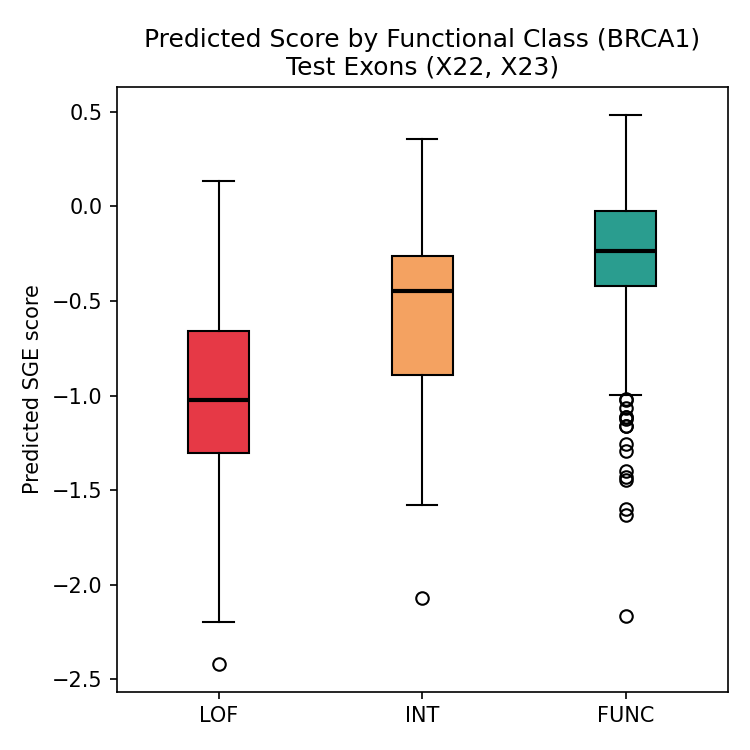
\includegraphics[width=\textwidth]{figures/sge_regressor_boxplot.png}
  \caption{BRCA1 predicted score by functional class on test exons X22--X23.}
  \label{fig:brca1_box}
\end{subfigure}
\caption{\textbf{BRCA1 SGE regressor performance on held-out test exons (X22--X23).}}
\label{fig:brca1_results}
\end{figure}

\begin{figure}[ht]
\centering
\begin{subfigure}[b]{0.48\textwidth}
  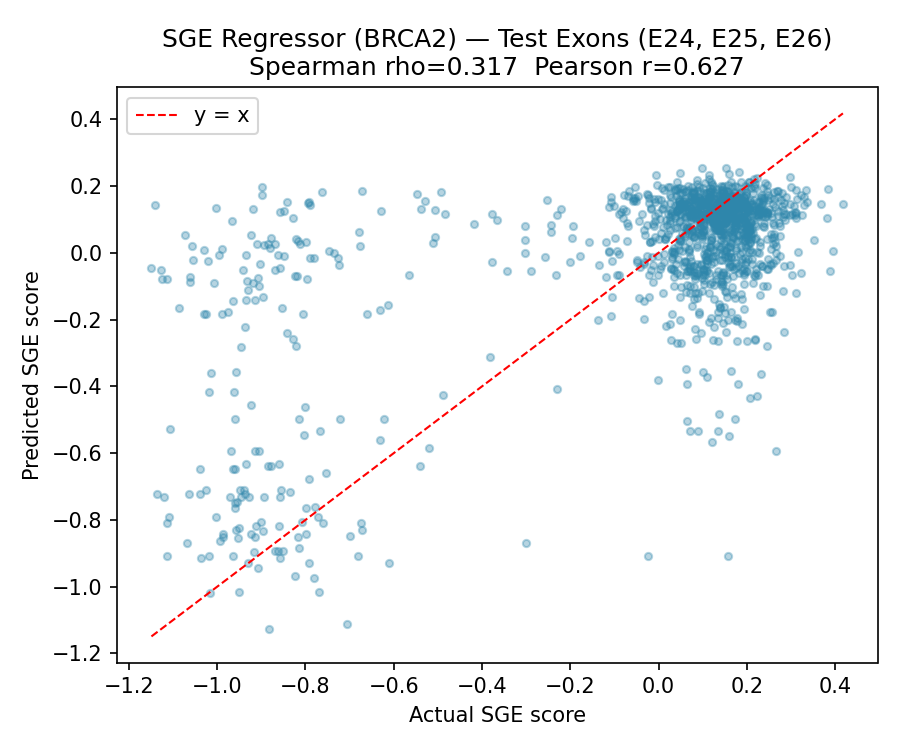
\includegraphics[width=\textwidth]{figures/sge_regressor_scatter_brca2.png}
  \caption{BRCA2 scatter: predicted vs actual SGE score.
           Spearman $\rho = 0.317$, Pearson $r = 0.627$.}
  \label{fig:brca2_scatter}
\end{subfigure}
\hfill
\begin{subfigure}[b]{0.48\textwidth}
  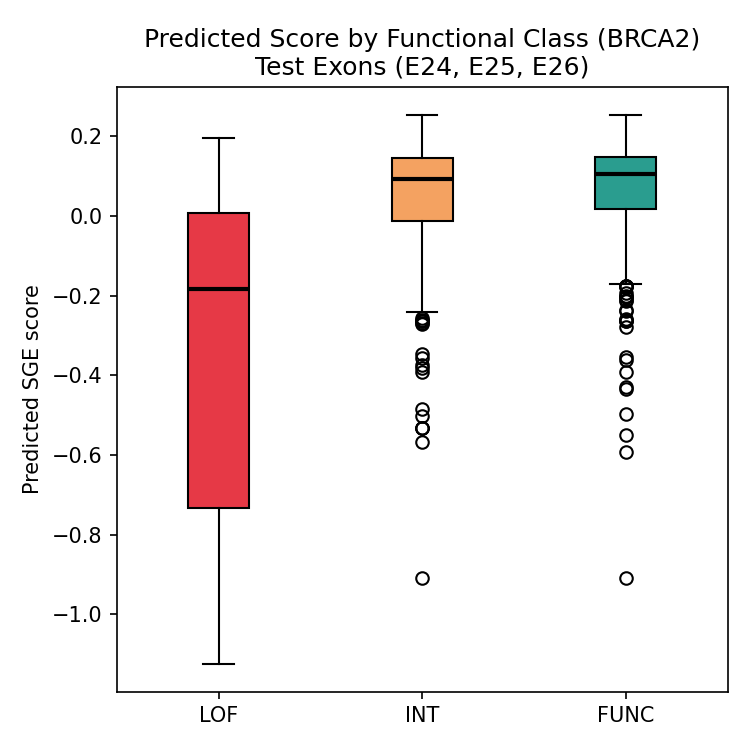
\includegraphics[width=\textwidth]{figures/sge_regressor_boxplot_brca2.png}
  \caption{BRCA2 predicted score by functional class on test exons E24--E26.}
  \label{fig:brca2_box}
\end{subfigure}
\caption{\textbf{BRCA2 SGE regressor performance on held-out test exons (E24--E26).}}
\label{fig:brca2_results}
\end{figure}

\begin{figure}[ht]
\centering
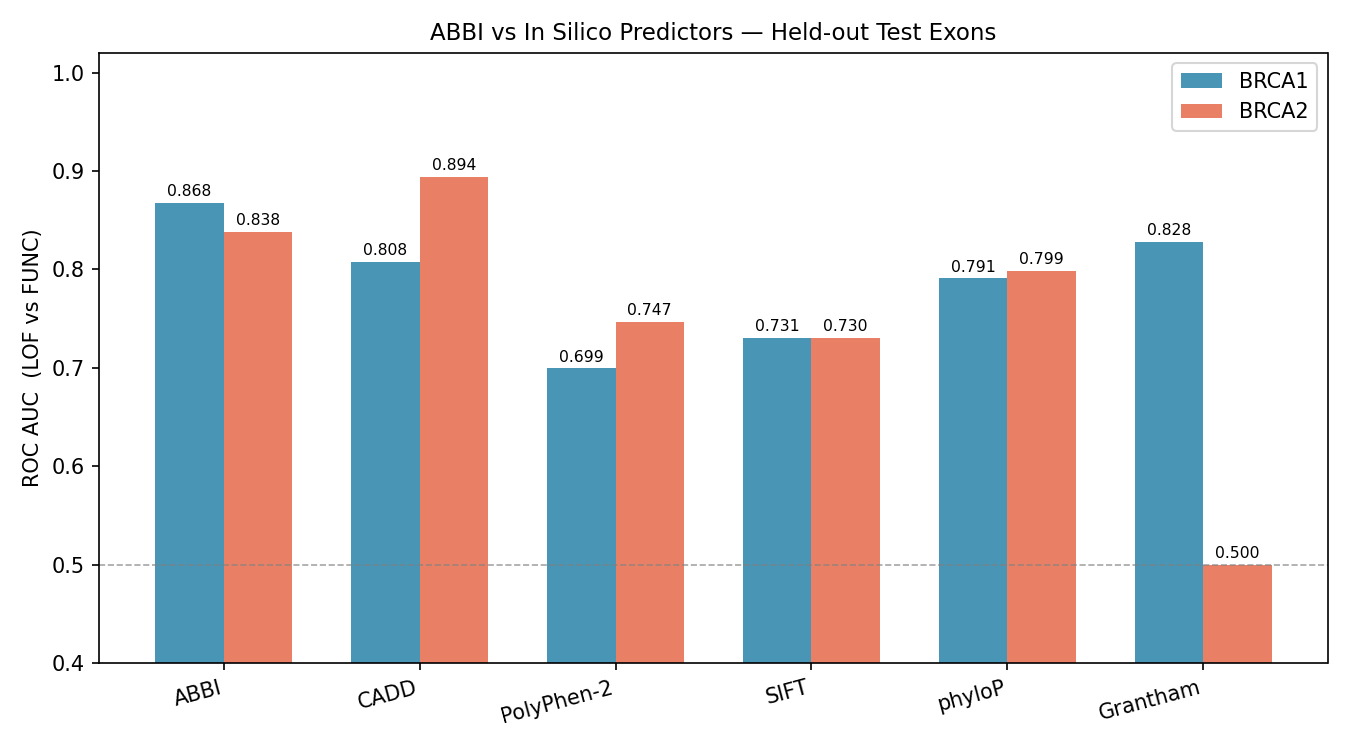
\includegraphics[width=0.75\textwidth]{figures/baseline_comparison.png}
\caption{\textbf{Baseline comparison.}
  ROC AUC (LOF vs FUNC) on held-out test exons for \abbi{} and five standard in silico
  predictors.
  \abbi{} leads on BRCA1; CADD leads on BRCA2, likely reflecting CADD's larger and more
  diverse training data.
  PolyPhen-2 and SIFT are evaluated on missense variants only.}
\label{fig:baselines}
\end{figure}

\end{document}
